%=============================================================
%  Entanglement Dynamics in a Spin-Chain Quantum Channel
%  Full scientific report — ready for Overleaf
%=============================================================
\documentclass[12pt,a4paper]{article}

%-------------------------------------------------------------
% ENCODING & FONTS
%-------------------------------------------------------------
\usepackage[T1]{fontenc}
\usepackage[utf8]{inputenc}
\usepackage{lmodern}
\usepackage{microtype}

%-------------------------------------------------------------
% PAGE LAYOUT
%-------------------------------------------------------------
\usepackage[top=2.5cm,bottom=2.5cm,left=3cm,right=3cm]{geometry}
\usepackage{setspace}
\onehalfspacing

%-------------------------------------------------------------
% MATHEMATICS
%-------------------------------------------------------------
\usepackage{amsmath,amssymb,amsfonts,mathtools}
\usepackage{bm}
\usepackage{physics}   % \ket{}, \bra{}, \braket{}{}, \Tr, \comm{}{}, \ev{}, etc.

%-------------------------------------------------------------
% GRAPHICS & DIAGRAMS
%-------------------------------------------------------------
\usepackage{graphicx}
\usepackage{tikz}
\usetikzlibrary{arrows.meta, positioning, decorations.pathreplacing, calc}
\usepackage{subcaption}

%-------------------------------------------------------------
% TABLES
%-------------------------------------------------------------
\usepackage{booktabs}
\usepackage{array}

%-------------------------------------------------------------
% ALGORITHM / PSEUDOCODE
%-------------------------------------------------------------
\usepackage[ruled,vlined,linesnumbered]{algorithm2e}
\SetKwComment{Comment}{$\triangleright$\ }{}

%-------------------------------------------------------------
% REFERENCES & LINKS
%-------------------------------------------------------------
\usepackage[numbers,sort&compress]{natbib}
\usepackage[colorlinks=true,
            linkcolor=blue!70!black,
            citecolor=blue!70!black,
            urlcolor=blue!70!black]{hyperref}
\usepackage{doi}   % defines \doi{text} -> \href{https://doi.org/text}{text}

%-------------------------------------------------------------
% MISCELLANEOUS
%-------------------------------------------------------------
\usepackage{xcolor}
\usepackage{enumitem}
\usepackage{float}

%-------------------------------------------------------------
% CUSTOM MATH COMMANDS
%-------------------------------------------------------------
\newcommand{\Ham}{\hat{H}}
\newcommand{\rhohat}{\hat{\rho}}
\newcommand{\Hilb}{\mathcal{H}}
\newcommand{\sigx}{\hat{\sigma}^x}
\newcommand{\sigy}{\hat{\sigma}^y}
\newcommand{\sigz}{\hat{\sigma}^z}
\newcommand{\sigp}{\hat{\sigma}^+}
\newcommand{\sigm}{\hat{\sigma}^-}
\newcommand{\TrC}{\mathrm{Tr}_C}
\newcommand{\TrA}{\mathrm{Tr}_A}
\newcommand{\TrB}{\mathrm{Tr}_B}
\DeclareMathOperator{\diag}{diag}
\newcommand{\uparr}{\uparrow}
\newcommand{\downarr}{\downarrow}
% Override \Tr from physics to use upright font
\renewcommand{\Tr}{\mathrm{Tr}}

%=============================================================
\begin{document}
%=============================================================

\title{\textbf{Entanglement Dynamics of Two Spin-1/2 Particles\\
       Coupled Through an Open XXZ Spin Chain}}
\author{}
\date{\today}
\maketitle
\thispagestyle{empty}

%-------------------------------------------------------------
\begin{abstract}
We define the model and methodology for studying the time evolution of quantum
correlations between two spin-1/2 particles — hereafter called system spins $A$
and $B$ — each coupled by a flip-flop interaction to one end of an open
$L$-site XXZ spin chain.  The full composite system evolves unitarily under a
Hamiltonian that includes local fields on the system spins, the internal
XXZ exchange interactions of the chain with anisotropy parameter $\Delta$, and
the boundary couplings.  Starting from an initial state in which the two system
spins share a maximally entangled Bell state $\ket{\Phi^+}$ while the chain is
in a thermal state, the reduced
two-spin density matrix $\rhohat_{AB}(t)$ is obtained at each time step by
tracing out the chain.  Eight quantum information and fidelity measures are
defined and tracked as functions of time: purity, the von Neumann entropies of
each subsystem and of the pair, the quantum mutual information, the Wootters
concurrence, and the spin-pair and global survival probabilities.  The
computation is based on an exact spectral decomposition of the full Hamiltonian.  A complementary
characterisation of the boundary-induced dynamical map via its
Choi--Jamio{\l}kowski representation is also presented.  The framework supports a parameter sweep
over chain length $L\in\{3,\ldots,7\}$ and anisotropy $\Delta\in[0.5,1.5]$.
\end{abstract}

\newpage
\tableofcontents
\newpage

%=============================================================
\section{Introduction}
\label{sec:intro}
%=============================================================
Spin chains, with their nearest-neighbour
exchange interactions and natural one-dimensional geometry, have been extensively
studied as models for quantum wires capable of mediating entanglement between
remote qubits~\cite{bose2003,christandl2004prl,christandl2005pra,osborne2004,subrahmanyam2004,bose2007review,Bayat2005,NielsenChuang2000}.  In this setting, two
spin-1/2 particles — the ``sender'' and ``receiver'' of quantum information —
are attached to the ends of a spin chain that serves as the quantum channel.
The chain's internal dynamics, together with the strength and form of its
boundary couplings, determine how quantum correlations are transported, degraded,
or redistributed over time~\cite{burgarth2005,wojcik2005,venuti2006,yung2005,godsil2012,cai2006decoherence,bayat2008memory,qin2013thermal}.

The present work focuses on the entanglement dynamics of this system in the
fully closed (unitary) regime.  We consider two spin-1/2 particles coupled
through a flip-flop interaction to the boundary sites of an open XXZ chain of
length $L$.  The key diagnostic object is the reduced density matrix
$\rhohat_{AB}(t)$ of the two system spins, obtained by tracing out the chain
from the full evolved state.  From $\rhohat_{AB}(t)$, several well-established
quantum information measures are computed, each capturing a different aspect of
the two-spin correlations as they evolve under the many-body dynamics of the
chain.

The primary physical questions motivating this study are: (i) how does the
entanglement between the two system spins decay and potentially revive as a
function of time, (ii) how do the chain length $L$ and the XXZ anisotropy
$\Delta$ influence this dynamics?

%=============================================================
\section{Physical Model}
\label{sec:model}
%=============================================================

\subsection{Hilbert Space and Site Layout}
\label{subsec:hilbert}

The composite system consists of three parts: system spin $A$, the $L$-site spin
chain $C$, and system spin $B$.  Each spin-1/2 particle lives in a two-dimensional
complex Hilbert space $\mathbb{C}^2$, spanned by the eigenstates
$\{\ket{\uparr},\ket{\downarr}\}$ of $\sigz$ with eigenvalues $+1$ and $-1$
respectively.  The total Hilbert space is
\begin{equation}
  \Hilb \;=\; \Hilb_A \otimes \Hilb_C \otimes \Hilb_B,
  \qquad \Hilb_A \cong \Hilb_B \cong \mathbb{C}^2,
  \qquad \Hilb_C \cong \bigl(\mathbb{C}^2\bigr)^{\otimes L},
  \label{eq:hilbert}
\end{equation}
with total dimension $D \equiv \dim\Hilb = 2^{L+2}$.  Throughout this work the
ordering $[A,\, C,\, B]$ is maintained: spin $A$ occupies the leftmost tensor
factor, the chain $C$ occupies the middle $L$ factors, and spin $B$ occupies
the rightmost factor.

The physical layout is illustrated in Fig.~\ref{fig:setup}: spin $A$ is coupled
exclusively to chain site $1$ and spin $B$ to chain site $L$.

\begin{figure}[htbp]
\centering
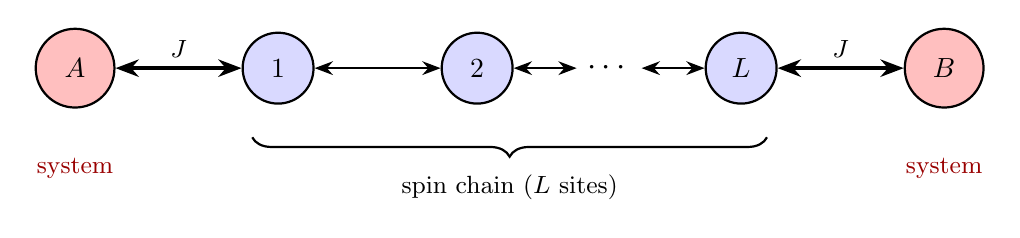
\begin{tikzpicture}[>=Stealth, thick, node distance=1.6cm]
  % System spin A
  \node[draw, circle, fill=red!25, minimum size=1.0cm, font=\bfseries] (A) {$A$};
  % Chain sites
  \node[draw, circle, fill=blue!15, minimum size=0.9cm, right=of A] (c1) {$1$};
  \node[draw, circle, fill=blue!15, minimum size=0.9cm, right=of c1] (c2) {$2$};
  \node[right=0.8cm of c2, font=\large] (dots) {$\cdots$};
  \node[draw, circle, fill=blue!15, minimum size=0.9cm, right=0.8cm of dots] (cL) {$L$};
  % System spin B
  \node[draw, circle, fill=red!25, minimum size=1.0cm, right=of cL,
        font=\bfseries] (B) {$B$};
  % Edges
  \draw[<->, very thick] (A) -- node[above,font=\small]{$J$} (c1);
  \draw[<->] (c1) -- (c2);
  \draw[<->] (c2) -- (dots);
  \draw[<->] (dots) -- (cL);
  \draw[<->, very thick] (cL) -- node[above,font=\small]{$J$} (B);
  % Chain brace
  \draw[decorate,decoration={brace,amplitude=7pt,mirror}]
    ([yshift=-0.55cm]c1.south west) -- ([yshift=-0.55cm]cL.south east)
    node[midway,below=10pt,font=\small]{spin chain ($L$ sites)};
  % Labels below system spins
  \node[below=0.5cm of A, font=\small,text=red!60!black] {system};
  \node[below=0.5cm of B, font=\small,text=red!60!black] {system};
\end{tikzpicture}
\caption{Physical setup.  System spins $A$ and $B$ (red) are each coupled to
one end of an $L$-site open XXZ spin chain (blue) via a flip-flop interaction of
strength $J$.  The chain mediates the interaction between the two distant system
spins.}
\label{fig:setup}
\end{figure}

\subsection{The Spin Chain: Open XXZ Model}
\label{subsec:xxz}

The internal dynamics of the chain is governed by the open XXZ Hamiltonian with
boundary fields~\cite{Bayat2005}:

\begin{equation}
  \Ham_C \;=\; -\frac{1}{2}\sum_{n=1}^{L-1}
    \Bigl[\sigx_n\sigx_{n+1} + \sigy_n\sigy_{n+1}
          + \Delta\bigl(\sigz_n\sigz_{n+1} - \mathbb{I}\bigr)\Bigr]
    - \frac{h_1}{2}\sigz_1 - \frac{h_2}{2}\sigz_L
    + \frac{h_1+h_2}{2}\,\mathbb{I}_C.
  \label{eq:Hchain}
\end{equation}

Here $\sigx_n, \sigy_n, \sigz_n$ are the Pauli matrices acting on site $n$ of the
chain (identity on all other chain sites), $\mathbb{I}_C$ is the identity on $\Hilb_C$,
$\Delta\in\mathbb{R}$ is the anisotropy parameter, and $h_1, h_2\in\mathbb{R}$
are the magnetic boundary fields applied to the first and last chain sites
respectively.  The constant term $(h_1{+}h_2)/2\cdot\mathbb{I}_C$ shifts the
zero-field energy to a convenient reference.

The anisotropy $\Delta$ controls the relative weight of the Ising ($\sigz\sigz$)
term relative to the isotropic XY exchange: at $\Delta=0$ the model is a free
XX chain; at $\Delta=1$ it is the isotropic Heisenberg (XXX) model; for
$\Delta>1$ the Ising interaction dominates.

\subsection{Boundary Couplings}
\label{subsec:coupling}

System spin $A$ is coupled to chain site $1$, and system spin $B$ to chain site
$L$, through \emph{flip-flop} (XX+YY) interactions:
\begin{align}
  \Ham_{AC} &= J\,\bigl(
    \sigp_A \otimes \sigm_{c,1} \otimes \mathbb{I}_B
    + \sigm_A \otimes \sigp_{c,1} \otimes \mathbb{I}_B
  \bigr), \label{eq:HAC}\\[4pt]
  \Ham_{CB} &= J\,\bigl(
    \mathbb{I}_A \otimes \sigp_{c,L} \otimes \sigm_B
    + \mathbb{I}_A \otimes \sigm_{c,L} \otimes \sigp_B
  \bigr), \label{eq:HCB}
\end{align}
where $\sigp_{c,1} = \sigp\otimes\mathbb{I}^{\otimes(L-1)}$ (raising operator at site
$1$ of the chain, identity elsewhere in $\Hilb_C$), $\sigm_{c,1}$ its
Hermitian conjugate, and $\sigp_{c,L} = \mathbb{I}^{\otimes(L-1)}\otimes\sigp$ for
site $L$.  The coupling $J > 0$ is the same at both boundaries.

The flip-flop interaction conserves total magnetisation
$M = \sigz_A + \sum_n\sigz_n + \sigz_B$: the operator $[\Ham_{AC}, M] = 0$,
ensuring that spin-excitation number is preserved during the dynamics.

\subsection{Local System Hamiltonians}
\label{subsec:local}

Each system spin is subject to a local longitudinal (Zeeman) field:
\begin{align}
  \Ham_A &= \Delta_A\,\sigz_A \otimes \mathbb{I}_C \otimes \mathbb{I}_B, \label{eq:HA}\\
  \Ham_B &= \mathbb{I}_A \otimes \mathbb{I}_C \otimes \Delta_B\,\sigz_B. \label{eq:HB}
\end{align}

\subsection{Full Hamiltonian}
\label{subsec:fullH}

Combining all terms, the total Hamiltonian of the composite system is
\begin{equation}
  \boxed{
    \Ham = \Ham_A + \mathbb{I}_A\otimes\Ham_C\otimes\mathbb{I}_B + \Ham_B
           + \Ham_{AC} + \Ham_{CB},
  }
  \label{eq:Htotal}
\end{equation}
acting on $\Hilb = \Hilb_A\otimes\Hilb_C\otimes\Hilb_B$.  The Hamiltonian is
Hermitian by construction and generates a unitary time evolution.

%The numerical parameters used in this study are collected in
%Table~\ref{tab:params}.

% BEGIN COMMENTED OUT BY REQUEST
%\begin{table}[htbp]
%\centering
%\caption{Numerical parameters.  The coupling strength in the code uses the
%convention $\hat{\sigma}^\pm_{\text{code}} = \hat{\sigma}^x \pm i\hat{\sigma}^y
%= 2\hat{\sigma}^\pm$; hence $J = 4\lambda$ where $\lambda=0.35$ is the
%code parameter (see Appendix~\ref{app:convention}).}
%\label{tab:params}
%\begin{tabular}{llcl}
%\toprule
%\textbf{Quantity} & \textbf{Symbol} & \textbf{Value} & \textbf{Notes}\\
%\midrule
%Local field, spin $A$  & $\Delta_A$ & $1.0$  & fixed \\
%Local field, spin $B$  & $\Delta_B$ & $1.0$  & fixed \\
%Boundary coupling      & $J$         & $1.4$  & $J=4\lambda$, $\lambda=0.35$ \\
%Left boundary field    & $h_1$       & $0.99$ & fixed \\
%Right boundary field   & $h_2$       & $1.01$ & fixed \\
%Anisotropy (swept)     & $\Delta$    & $[0.5,\,1.5]$ step $0.1$ \\
%Chain length (swept)   & $L$         & $\{3,4,5,6,7\}$ & 6 values \\
%Time range             & $t_{\max}$  & $50$ & $\delta t = 0.1$ \\
%\bottomrule
%\end{tabular}
%\end{table}
% END COMMENTED OUT BY REQUEST

The slight asymmetry $h_1 \neq h_2$ lifts the left-right reflection symmetry of
the chain, breaking potential degeneracies and ensuring a generically non-degenerate spectrum — a standard regularisation in numerical studies of spin transport. Although, for the numerical results presented later this point was not verified rigurosly.

%=============================================================
\section{Initial State}
\label{sec:initial}
%=============================================================

The initial state of the full system is assumed to be a \emph{tensor product}
between the two-spin state and the chain state:
\begin{equation}
  \rhohat(0) = \rhohat_{AB}(0)\otimes\rhohat_C(0).
  \label{eq:rho0}
\end{equation}
This factored form is the only structural assumption on the initial state; the
individual components $\rhohat_{AB}(0)$ and $\rhohat_C(0)$ can each be any
valid density matrix on their respective spaces.

\paragraph{Two-spin initial state.}
The system spins are initialised in the maximally entangled \emph{Bell state}
\begin{equation}
  \ket{\Phi^+} = \frac{1}{\sqrt{2}}\,\bigl(\ket{\uparr\uparr} + \ket{\downarr\downarr}\bigr),
  \qquad
  \rhohat_{AB}(0) = \ketbra{\Phi^+}{\Phi^+}.
  \label{eq:bell}
\end{equation}
In the computational basis $\{\ket{\uparr\uparr},\ket{\uparr\downarr},
\ket{\downarr\uparr},\ket{\downarr\downarr}\}$, the density matrix reads
\begin{equation}
  \rhohat_{AB}(0) = \frac{1}{2}\begin{pmatrix}1&0&0&1\\0&0&0&0\\0&0&0&0\\1&0&0&1\end{pmatrix}.
  \label{eq:rhoAB0}
\end{equation}
This is a pure state ($\Tr[\rhohat_{AB}^2(0)]=1$) with Wootters concurrence
$\mathcal{C}=1$, i.e.\ maximum two-qubit entanglement.


\paragraph{Chain initial state.}
The chain is initialised in a thermal Gibbs state at inverse temperature
$\beta=1/(k_B T)$:
\begin{equation}
  \rhohat_C(0) = \rhohat_C^{(\beta)}
  = \frac{e^{-\beta \Ham_C}}{Z_C(\beta)},
  \qquad
  Z_C(\beta) = \Tr_C\!\left(e^{-\beta \Ham_C}\right).
  \label{eq:rhoC0}
\end{equation}
Here $Z_C(\beta)$ is the chain partition function, ensuring
$\Tr_C[\rhohat_C(0)]=1$.  The zero-temperature limit $\beta\to\infty$ projects
onto the ground-state subspace of $\Ham_C$, while the infinite-temperature limit
$\beta\to0$ gives the maximally mixed chain state $\rhohat_C(0)=\mathbb{I}_C/2^L$.

\paragraph{Full initial state.}
Combining Eqs.~\eqref{eq:bell}--\eqref{eq:rhoC0} via Eq.~\eqref{eq:rho0} and
permuting to the $[A,C,B]$ tensor ordering (see
Appendix~\ref{app:permutation}) yields the $D\times D$ density matrix
$\rhohat(0)$ used in all computations.

%=============================================================
\section{Unitary Time Evolution}
\label{sec:evolution}
%=============================================================

The composite system evolves under the von Neumann equation (with $\hbar=1$)
\begin{equation}
  \frac{d\rhohat}{dt} = -i[\Ham,\rhohat],
  \label{eq:vonNeumann}
\end{equation}
whose formal solution is
\begin{equation}
  \rhohat(t) = e^{-i\Ham t}\,\rhohat(0)\,e^{+i\Ham t}.
  \label{eq:rho_t}
\end{equation}
Since $\Ham$ is a finite $D\times D$ Hermitian matrix, the time evolution
operator $e^{-i\Ham t}$ can be evaluated exactly through spectral decomposition.

Let $\{\ket{E_\alpha}\}_{\alpha=1}^D$ be the complete orthonormal set of
eigenvectors of $\Ham$ with corresponding eigenvalues $E_1\leq E_2\leq\cdots\leq E_D$.
Defining the unitary matrix $U$ with elements $U_{\alpha j} = \braket{E_\alpha|j}$
(rows of $U$ are eigenvectors), the density matrix in the energy basis is

\begin{equation}
  [\rho_E]_{\alpha\beta} \;=\; \braket{E_\alpha|\rhohat(0)|E_\beta}
  \;=\; [U\,\rhohat(0)\,U^\dagger]_{\alpha\beta}.
  \label{eq:rhoE}
\end{equation}

Under time evolution, the energy-basis matrix acquires simple phase factors:

\begin{equation}
  [\rho_E(t)]_{\alpha\beta} = [\rho_E]_{\alpha\beta}\,e^{-i(E_\alpha-E_\beta)t}.
  \label{eq:rhoE_t}
\end{equation}
The full state is recovered by $\rhohat(t) = U^\dagger\rho_E(t)\,U$.  Since no
matrix exponential or time-step integration is needed — only a Hadamard product
with phase factors — this representation is both exact and computationally
efficient.

\textit{Remark.}  Because the evolution is unitary with the total Hamiltonian there could be potentially several degeneracies which were not analyzed to perform the evolution due to the several parameters used. In addition to that, the terms appearing in equation~\ref{eq:rhoE} are almost the Krauss operators which forms the quantum channel.


%=============================================================
\section{Quantum Information Measures}
\label{sec:measures}
%=============================================================

As the chain becomes entangled with the system spins through the boundary
couplings, all diagnostics of the two-spin correlations are computed from the
\emph{reduced density matrix} $\rhohat_{AB}(t)$, obtained by tracing out the
chain.  This $4\times 4$ matrix is the fundamental object from which all
observables are derived.

\subsection{Reduced Density Matrix and Partial Trace}
\label{subsec:rdm}

For a bipartite quantum system $AB\cup C$ in state $\rhohat$, the
\emph{reduced density matrix} of the $AB$ subsystem is obtained by performing
the \emph{partial trace} over the environment $C$:
\begin{equation}
  \rhohat_{AB}(t) \;\equiv\; \Tr_C\!\bigl[\rhohat(t)\bigr]
  \;=\; \sum_{c=0}^{2^L-1}\bra{c}_C\,\rhohat(t)\,\ket{c}_C,
  \label{eq:rdm}
\end{equation}
where $\{\ket{c}_C\}$ is any orthonormal basis of $\Hilb_C$.  The
result is a $4\times4$ positive semidefinite Hermitian matrix satisfying
$\Tr[\rhohat_{AB}]=1$.  Although $\rhohat(0)$ is pure
[$\Tr(\rhohat^2(0))=1$], $\rhohat_{AB}(t)$ will generally be \emph{mixed}
for $t>0$, reflecting the build-up of entanglement between the system spins
and the chain.

In the $[A,C,B]$ tensor layout, the matrix elements are given explicitly by
\begin{equation}
  [\rhohat_{AB}(t)]_{(q_Aq_B),\,(q_A'q_B')}
  = \sum_{c=0}^{2^L-1}[\rhohat(t)]_{(q_A,c,q_B),\,(q_A',c,q_B')},
  \label{eq:ptrace_elements}
\end{equation}
where the compound index $(q_A, c, q_B)$ labels the computational basis element
in the full tensor product space.  All quantum information measures below are
computed from this $4\times4$ matrix.

\subsection{Purity}
\label{subsec:purity}

The \emph{purity} of the reduced state $\rhohat_{AB}(t)$ is
\begin{equation}
  \mathcal{P}(t) = \Tr\!\bigl[\rhohat_{AB}^2(t)\bigr].
  \label{eq:purity}
\end{equation}
For any density matrix on a $d$-dimensional space, $1/d \leq \mathcal{P} \leq 1$.
Purity equals $1$ if and only if the state is pure; purity $1/d$ corresponds to
the maximally mixed state.  At $t=0$ one has $\mathcal{P}(0)=1$ since
$\rhohat_{AB}(0)=\ketbra{\Phi^+}{\Phi^+}$ is pure.  As the system spins become
entangled with the chain, $\mathcal{P}(t)$ decreases.  A sudden drop to small
values indicates rapid decoherence driven by the chain.

\subsection{Von Neumann Entropy}
\label{subsec:vne}

The \emph{von Neumann entropy} of a density matrix $\rhohat$ is the quantum
generalisation of the Shannon entropy of a probability distribution:
\begin{equation}
  S(\rhohat) = -\Tr[\rhohat\ln\rhohat] = -\sum_k \lambda_k\ln\lambda_k,
  \label{eq:vne}
\end{equation}
where $\{\lambda_k\}$ are the eigenvalues of $\rhohat$, and the convention
$0\cdot\ln 0 \equiv 0$ is adopted.  The natural logarithm is used throughout,
giving entropies in \emph{nats} ($1\,\text{nat}\approx 1.443\,\text{bits}$).
The von Neumann entropy is non-negative, vanishes if and only if $\rhohat$ is a
pure state, and reaches its maximum value $\ln d$ for the maximally mixed state
on a $d$-dimensional space.

Three entropies are computed at each time step:
\begin{enumerate}[label=(\roman*)]
  \item \textbf{Entropy of spin $A$}:
        $S_A(t) = S(\rhohat_A(t))$,
        where $\rhohat_A(t) = \Tr_B[\rhohat_{AB}(t)]$ is the $2\times2$
        single-spin reduced state of $A$.
  \item \textbf{Entropy of spin $B$}:
        $S_B(t) = S(\rhohat_B(t))$,
        where $\rhohat_B(t) = \Tr_A[\rhohat_{AB}(t)]$.
  \item \textbf{Entropy of the spin pair}:
        $S_{AB}(t) = S(\rhohat_{AB}(t))$,
        computed from the full $4\times4$ reduced matrix.
\end{enumerate}
At $t=0$: $S_{AB}(0)=0$ (pure state), but
$S_A(0) = S_B(0) = \ln 2 \approx 0.693$ nats (maximal single-qubit entropy,
reflecting the perfect entanglement of the Bell state).

\subsection{Quantum Mutual Information}
\label{subsec:mi}

The \emph{quantum mutual information} between spins $A$ and $B$ is defined as
\begin{equation}
  I(A{:}B)(t) = S_A(t) + S_B(t) - S_{AB}(t).
  \label{eq:mi}
\end{equation}
For any state $\rhohat_{AB}$, one has $I(A{:}B) \geq 0$, with equality if and
only if $\rhohat_{AB} = \rhohat_A\otimes\rhohat_B$ (no correlations whatsoever).
The mutual information captures \emph{all} correlations between $A$ and $B$ —
both classical and quantum.  It can be nonzero for states that have zero
entanglement, whenever they carry classical correlations.  At $t=0$,
$I(A{:}B)(0) = 2\ln2 \approx 1.386$ nats, the maximum possible for a two-qubit
pure state.

An important conceptual point: $I(A{:}B)$ is computed from the \emph{marginal}
state $\rhohat_{AB}$, from which the chain has been traced out.  It therefore
measures only the correlations between $A$ and $B$ as seen by an observer with
no access to the chain, and does not capture correlations that exist within the
tripartite structure of the full state.

\subsection{Wootters Concurrence}
\label{subsec:concurrence}

For a general two-qubit (mixed) state $\rhohat_{AB}$, the \emph{entanglement of
formation} $E_F$ quantifies the minimum entanglement needed to prepare
$\rhohat_{AB}$ as a convex mixture of pure states~\cite{NielsenChuang2000}.
Wootters showed that $E_F$ is an increasing function of the \emph{concurrence}
$\mathcal{C}$, defined as follows.  Let
\begin{equation}
  \tilde{\rho} = (\sigy\otimes\sigy)\,\rhohat_{AB}^*\,(\sigy\otimes\sigy),
  \label{eq:rhotilde}
\end{equation}
where $\rhohat_{AB}^*$ denotes the complex conjugate in the standard basis and
$\sigy\otimes\sigy$ is the two-qubit spin-flip operator.  Let
$\lambda_1\geq\lambda_2\geq\lambda_3\geq\lambda_4\geq0$ be the square roots of
the eigenvalues of the product $\rhohat_{AB}\,\tilde{\rho}$.  Then
\begin{equation}
  \mathcal{C}(\rhohat_{AB}) = \max\!\bigl(0,\,\lambda_1-\lambda_2-\lambda_3-\lambda_4\bigr).
  \label{eq:concurrence}
\end{equation}
The concurrence ranges from $0$ (separable state, no entanglement) to $1$
(maximally entangled state).  For the initial Bell state,
$\mathcal{C}(0) = 1$.

The concurrence is an entanglement measure for the \emph{marginal} state
$\rhohat_{AB}$, not for the full tripartite state.  Due to the monogamy of
entanglement, as spin $A$ becomes increasingly entangled with the chain,
$\mathcal{C}(\rhohat_{AB})$ decreases.  Reaching $\mathcal{C}=0$ at a finite
time (entanglement sudden death) signals complete loss of pairwise entanglement
between $A$ and $B$ in the marginal picture, even though quantum discord between
them may remain nonzero.

\subsection{Spin-Pair Survival Probability}
\label{subsec:survival}

The \emph{spin-pair survival probability} (or spin-pair fidelity) measures how
close the current reduced state $\rhohat_{AB}(t)$ is to the initial two-spin
state $\rhohat_{AB}(0)$:
\begin{equation}
  F_{AB}(t) = \Tr\!\bigl[\rhohat_{AB}(0)\,\rhohat_{AB}(t)\bigr].
  \label{eq:spin_survival}
\end{equation}
Since $\rhohat_{AB}(0)=\ketbra{\Phi^+}{\Phi^+}$ is pure, this simplifies to the
overlap
\begin{equation}
  F_{AB}(t) = \bra{\Phi^+}\rhohat_{AB}(t)\ket{\Phi^+},
  \label{eq:spin_survival_pure}
\end{equation}
i.e.\ the probability of finding the spin pair in its original Bell state at
time $t$.  $F_{AB}(0)=1$ by definition, and generally $F_{AB}(t) < 1$ for
$t > 0$.

\subsection{Global Survival Probability}
\label{subsec:global}

The \emph{global survival probability} measures the fidelity of the \emph{full}
many-body state $\rhohat(t)$ with respect to the initial state $\rhohat(0)$:

\begin{equation}
  F_{\mathrm{glob}}(t) = \Tr\!\bigl[\rhohat(0)\,\rhohat(t)\bigr].
  \label{eq:global_survival}
\end{equation}

For a pure states, this reduces to the usual
$F_{\mathrm{glob}}(t)=|\langle\psi(0)|\psi(t)\rangle|^2$.  With a thermal chain state,
$\rhohat(0)$ is generally mixed, so Eq.~\eqref{eq:global_survival} should be
interpreted as a Hilbert--Schmidt overlap rather than a normalized survival
probability; in particular, $F_{\mathrm{glob}}(0)=\Tr[\rhohat(0)^2]$ equals the
initial full-state purity.

This global overlap complements the spin-pair survival: while $F_{AB}$ asks
whether the two system spins have retained their original correlations,
$F_{\mathrm{glob}}$ asks how far the entire composite state (spins plus chain)
has moved away from its initial thermal preparation.


\subsection{Some results}

Here I'm showing only two plots of all the results that are avaliable here \url{https://github.com/MiguelICN/Spin-transport/tree/main}. I made a sweep across $\Delta$ but the results do not change significantly, for every parameter several values of $\beta$ were used for the initial state of the environment. You'll also find a sweep for several sizes from $L=3-7$. The initial state for the boundary spins was a Bell state. The most important conclusion is that entanglement of one spin vs the other partition almost remains constant. This is because the spin stops being entangled with the other spin but it gets entangled with the chain. The spin survival is for the joint system. The purity is computed for the joint system, spin A-B, so it is a direct measure of (linear entropy) entanglement between the joint system and the chain. In the repository you can consult another set of results for $\lambda_A = \lambda_B = 0.1$, which corresponds to a somewhat weak cooupling limit.
 
\begin{figure}[htbp]
  \centering
  \includegraphics[width=\textwidth]{Figures/AllObservables_D10_bInf.png}
  \caption{In this figure it is shown several quantum information measures with all relevant parameters are equal to 1 for the XXZ model with open boundary conditions and $L=7$. The initial state of the environment has $\beta = \infty$, so it is the ground state of the chain.}
  \label{fig:observables_beta_inf}
\end{figure}

\begin{figure}[htbp]
  \centering
  \includegraphics[width=\textwidth]{Figures/AllObservables_D10_b0p0.png}
  \caption{In this figure it is shown several quantum information measures with all relevant parameters are equal to 1 for the XXZ model with open boundary conditions and $L=7$. The initial state of the environment has $\beta = 0$.}
  \label{fig:observables_beta_zero}
\end{figure}




\clearpage
\newpage
%=============================================================
\section{Quantum Channel}
\label{sec:quantum_channel}
%=============================================================

The previous sections provided the components to define the quantum channel which drives the evolution of the reduced density matrix of both boundary spins. In other words, the evolution of the reduced density matrix of the boundary spins is non-unitary in general, and this evolution is what defines the dynamical map.

A dynamical map is a CPTP map which depends parametrically on the time $t$ which comes from the continous time evolution of the total system. It is a map that comes from tracing out the spin chain degrees of freedom.

%=============================================================
\section{Choi-State Representation of the Boundary Dynamical Map}
\label{sec:choi}
%=============================================================

The reduced-state observables of Section~\ref{sec:measures} characterise the
trajectory $\rhohat_{AB}(t)$ for one fixed initial state $\rhohat_{AB}(0)$.
The boundary couplings $\Ham_{AC},\Ham_{CB}$ together with the chain define a
single object that is independent of this choice: the \emph{dynamical map}
$\mathcal{E}_t$ itself. This section defines its Choi-Jamio{\l}kowski
representation~\cite{NielsenChuang2000}; the explicit construction methods and algorithm are collected in the appendix.

\subsection{The Reduced Dynamical Map and Its Choi Matrix}
\label{subsec:choi_def}

Let $\Hilb_{AB}\equiv\Hilb_A\otimes\Hilb_B$, with $d_S\equiv\dim\Hilb_{AB}=4$,
and $d_E\equiv\dim\Hilb_C=2^L$, so that $D=d_Sd_E$. For a fixed initial chain
state $\rhohat_C(0)$, the chain-induced channel acting on the system spins is
\begin{equation}
  \mathcal{E}_t(\hat{O}) \;\equiv\;
  \TrC\!\Bigl[e^{-i\Ham t}\bigl(\hat{O}\otimes\rhohat_C(0)\bigr)e^{+i\Ham t}\Bigr],
  \qquad \hat{O}\in\mathcal{B}(\Hilb_{AB}),
  \label{eq:choi_channel}
\end{equation}
a completely positive, trace-preserving map. Setting $\hat O=\rhohat_{AB}(0)$
recovers $\rhohat_{AB}(t)$ of Eq.~\eqref{eq:rdm}; $\mathcal{E}_t$ is the
object that produces $\rhohat_{AB}(t)$ for \emph{every} possible system
input, in one shot.

Introduce an auxiliary reference space $\Hilb_R\cong\Hilb_{AB}$, an
orthonormal basis $\{\ket{i}\}_{i=1}^{d_S}$ of $\Hilb_{AB}$ in one-to-one
correspondence with the spin-pair labels already used in
Eq.~\eqref{eq:ptrace_elements}, $i\leftrightarrow(q_A^{(i)},q_B^{(i)})$ with
$i=2q_A^{(i)}+q_B^{(i)}+1$, and the maximally entangled state
\begin{equation}
  \ket{\Omega} = \frac{1}{\sqrt{d_S}}\sum_{i=1}^{d_S}\ket{i}_R\ket{i}_{AB}
  \quad\in\;\Hilb_R\otimes\Hilb_{AB}.
  \label{eq:choi_omega}
\end{equation}
($\ket{\Omega}$ is distinct from the physical Bell state $\ket{\Phi^+}$ of
Eq.~\eqref{eq:bell}; it is a fixed reference state with no role in the
dynamics.) The \emph{Choi matrix} of $\mathcal{E}_t$ is
\begin{equation}
  \hat{\chi}(t) \;\equiv\; (\mathrm{id}_R\otimes\mathcal{E}_t)\bigl(\ketbra{\Omega}{\Omega}\bigr)
  \;=\; \frac{1}{d_S}\sum_{i,j=1}^{d_S}\ketbra{i}{j}\otimes\mathcal{E}_t\bigl(\ketbra{i}{j}\bigr),
  \label{eq:choi_def}
\end{equation}
a $d_S^2\times d_S^2 = 16\times16$ positive semidefinite, unit-trace matrix
by the Choi--Jamio{\l}kowski isomorphism. Its eigenvalues are non-negative
and sum to $1$; $\Tr[\hat\chi^2(t)]$ and $S(\hat\chi(t))$ (Eq.~\eqref{eq:vne})
quantify, respectively, how close $\mathcal{E}_t$ is to a unitary (noiseless)
map and how much the chain has scrambled the channel by time $t$.

\subsection{Some results for the Choi state}

Using the same parameters as the ones for the observables for the reduced density matrix of the joint state of the spins, the following results are from the quantum channel which drives the evolution of the joint system. In this case, the quantum channel doesn't depend on the initial state of the joint system (the Bell state used for the earlier results).

\begin{figure}[h!]
  \centering
  \includegraphics[width=\textwidth]{Figures/ChoiObservables_D10_bInf.png}
  \caption{Choi state observables for the same parameters as the observables for the reduced density matrix used before, for $\beta=\infty$. The red dashed line is a bound for the purity.}
  
\end{figure}

\begin{figure}[h!]
  \centering
  \includegraphics[width=\textwidth]{Figures/ChoiEigenvalues5_D10_bInf.png}
  \caption{First five eigenvalues (out of 16) of the previous results. The sum squared of all eigenvalues make up the purity of the quantum channel ploted.}
  
\end{figure}



\begin{figure}[h!]
  \centering
  \includegraphics[width=\textwidth]{Figures/ChoiObservables_D10_b0p0.png}
  \caption{Choi state observables for the same parameters as the observables for the reduced density matrix used before for $\beta=0$}
  
\end{figure}

\begin{figure}[h!]
  \centering
  \includegraphics[width=\textwidth]{Figures/ChoiEigenvalues5_D10_b0p0.png}
  \caption{First five eigenvalues (out of 16) of the previous results. The sum squared of all eigenvalues make up the purity of the quantum channel ploted.}
  
\end{figure}

In this case, the results described the dynamics of the quantum channel of two qubits, so its interpretation is not as simple as for one qubit which are always deformation of the Bloch sphere. Similarly to the observables for the reduced density matrix, the oscillations get more damped the more energy differences are relevant to the computation, interpreted as equilibration. In the repository \url{https://github.com/MiguelICN/Spin-transport/tree/main} you can consult another set of results for $\lambda_A = \lambda_B = 0.1$.


\clearpage
%========================================================
\section{(Other possible quantifiers of) Quantum Information Transfer Through the Spin Chain}
\label{app:quantum_info_transfer}

Here are some potential candidates to use from the literature to quantify quantum information transmission from spin $Q_1$ to spin $Q_2$ mediated by the XXZ chain, and identifies which are directly accessible from the objects computed in this work.

\subsection{Quantum Channel Capacity}

The chain defines a quantum channel $\mathcal{E}_t$ acting on $Q_1$:
\begin{equation}
    \mathcal{E}_t(\rho_{Q_1}) =
    \mathrm{Tr}_{Q_2,\,\mathrm{chain}}\!\left[
        U(t)\,\bigl(\rho_{Q_1} \otimes \rho_{\mathrm{chain}}^{(\beta)}
        \otimes \rho_{Q_2}^{(0)}\bigr)\,U^\dagger(t)
    \right].
\end{equation}
The quantum capacity $Q(\mathcal{E})$ is the maximum asymptotic rate of reliable
quantum information transmission. It is bounded below by the \emph{coherent
information}~\cite{Schumacher1996,Lloyd1997}:
\begin{equation}
    I_c(\rho_{Q_1},\mathcal{E}) = S\!\left(\mathcal{E}_t(\rho_{Q_1})\right)
    - S_{Q_1 Q_2},
\end{equation}
where the second term is the entropy of the joint output state.

\subsection{Average State-Transfer Fidelity}

The most commonly reported diagnostic in the spin-chain literature~\cite{bose2003}
is the Haar-averaged fidelity of quantum state transfer:
\begin{equation}
    F(t) = \int d\psi\,\langle\psi|\,\rho_{Q_2}(t)\,|\psi\rangle,
\end{equation}
which for a qubit output reduces to a linear combination of two-point correlators
of $\rho_{Q_1 Q_2}(t)$. The threshold $F > 2/3$ marks the boundary above which
the channel surpasses any classical measure-and-prepare strategy, certifying
genuine quantum information transfer.

\subsection{Entanglement Fidelity and the Choi Matrix}

A channel transmits quantum information if and only if it can transmit
entanglement~\cite{Bennett1996,Horodecki1999}. This equivalence is made
operational through the \emph{entanglement fidelity}:
\begin{equation}
    F_e(t) = \langle\Phi^+|\,
    \bigl(\mathcal{I}_R \otimes \mathcal{E}_t\bigr)
    \bigl(|\Phi^+\rangle\langle\Phi^+|\bigr)
    \,|\Phi^+\rangle,
\end{equation}
where $|\Phi^+\rangle$ is a maximally entangled state of $Q_1$ with a reference
copy $R$, and $\mathcal{I}_R$ is the identity on $R$. This quantity is precisely
the overlap of the Choi matrix $\hat{\chi}(t)$ with the maximally entangled
projector, i.e.\ a direct linear functional of $\hat{\chi}(t)$. The average and
entanglement fidelities are related by~\cite{Nielsen2002}:
\begin{equation}
    F(t) = \frac{d\,F_e(t) + 1}{d + 1},
    \qquad d = 2.
\end{equation}

\subsection{Quantum Discord}

At finite temperature, quantum correlations in $\rho_{Q_1 Q_2}(t)$ may persist
below the entanglement threshold. \emph{Quantum discord}~\cite{Ollivier2001,Henderson2001}:
\begin{equation}
    D(Q_1|Q_2) = I(Q_1:Q_2) - J(Q_1|Q_2),
\end{equation}
where $I(Q_1:Q_2)$ is the quantum mutual information and $J(Q_1|Q_2)$ is the
classical mutual information optimised over measurements on $Q_2$, captures
quantum correlations beyond separability. $D > 0$ with $C = 0$ signals a regime
where the chain mediates sub-entanglement quantum correlations, relevant at high
temperature ($\beta \to 0$).

\subsection{Information Scrambling}

The tripartite mutual information:
\begin{equation}
    I_3(Q_1 : Q_2 : \mathrm{chain})
    = I(Q_1:Q_2) + I(Q_1:\mathrm{chain}) - I(Q_1: Q_2 \cup \mathrm{chain}),
\end{equation}
diagnoses whether information is \emph{transmitted} or \emph{scrambled}.
Negative $I_3$ indicates that information injected at $Q_1$ has been delocalized
into the chain bulk and is not accessible from either boundary alone.


%=============================================================
\section{Reference Discussion and Literature Context}
\label{app:references_discussion}
%=============================================================

The common thread across the following cited works is that a
many-body spin system can be treated not only as a Hamiltonian dynamics problem, but also as an induced quantum channel for a small set of endpoint degrees of freedom.  This perspective is especially useful here because the central object is the reduced map

\begin{equation}
  \rhohat_{AB}(t)
  = \Tr_C\!\left[U(t)\,\rhohat_{AB}(0)\otimes\rhohat_C(0)\,U^\dagger(t)\right],
  \qquad U(t)=e^{-i\Ham t},
  \label{app:reduced_map_context}
\end{equation}

which can also be represented as a completely positive trace-preserving map on
the endpoint pair.

\paragraph{Spin-chain communication and state transfer.}
The foundational state-transfer literature established that XX, XY, XXZ, and
Heisenberg-type chains can act as quantum wires, with performance controlled by
boundary conditions, coupling profiles, chain length, and readout time.  Bose's
unmodulated-chain proposal introduced the basic communication setting used by
many later works~\cite{bose2003}, while engineered couplings and perfect-transfer
networks were developed in Refs.~\cite{christandl2004prl,christandl2005pra}.
Related analyses of propagation, entanglement dynamics, conclusive transfer,
universal quantum wires, long-distance entanglement, and number-theoretic
transfer constraints appear in
Refs.~\cite{osborne2004,subrahmanyam2004,burgarth2005,wojcik2005,venuti2006,godsil2012}.
Together with the broader review literature~\cite{bose2007review}, these works
motivate the present use of endpoint observables, transfer times, and
correlation measures as diagnostics of a spin-chain channel.

\paragraph{Thermal and open-channel viewpoints.}
Bayat and Karimipour studied thermal effects on quantum communication through
spin chains using a reduced-channel formulation~\cite{Bayat2005}.  In that
setting the chain is initialized in a Gibbs state,
\begin{equation}
  \rhohat_C(0)=\frac{e^{-\beta\Ham_C}}{\Tr(e^{-\beta\Ham_C})},
  \label{app:gibbs_context}
\end{equation}
and the receiver or endpoint state is obtained after unitary evolution and a
partial trace over the remaining spins.  Their analysis shows how temperature
affects transfer fidelity and readout behavior, and it provides a close
methodological analogue of the reduced-state construction used in this report.
Subsequent work on decoherence in spin channels, repeated-use memory effects,
and finite-temperature transfer further supports treating transport quality,
entanglement transmission, and channel memory as map-level properties rather
than only as transition amplitudes~\cite{cai2006decoherence,bayat2008memory,qin2013thermal}.

\paragraph{Entanglement and correlation diagnostics.}
For two-qubit endpoint states, concurrence provides a direct measure of
bipartite entanglement and is computed using Wootters' closed formula for mixed
states~\cite{wootters1998}.  This is why concurrence is a sharper diagnostic of
direct $A$--$B$ entanglement than a single-spin entropy alone: $S(\rhohat_A)$ can
detect that spin $A$ is entangled with the rest of the tripartite system, but it
does not specify whether those correlations are with spin $B$ or with the chain.
The literature on finite-time disentanglement, often called entanglement sudden
death, shows that concurrence can vanish at finite times even when other
correlation measures decay more gradually~\cite{yu2004}.  This motivates the
simultaneous tracking of concurrence, mutual information, marginal entropies,
and purity in the main text.

\paragraph{Integrability, boundary impurities, and scalability.}
The present simulations use exact diagonalisation for finite $L$, but the notes
also point to larger-system directions.  For free-fermionic chains such as XX,
XY, or transverse-field Ising models, Jordan--Wigner methods can reduce the
problem to single-particle or covariance-matrix dynamics.  For interacting XXZ
chains, preserving exact integrability in the presence of boundary degrees of
freedom is more delicate.  Sklyanin's reflection-equation framework gives the
standard algebraic treatment of integrable boundaries~\cite{sklyanin1988}, and
related impurity constructions for Heisenberg and higher-spin chains are
discussed in Refs.~\cite{andrei1984,hou1999}.  These references are useful for
future extensions in which the endpoint spins are treated as integrable boundary
impurities rather than as generic external couplings.

% \paragraph{Research directions suggested by the literature.}
% Several extensions naturally follow from this combined reference set.  One is a
% benchmark of the integrable--chaotic crossover by adding random fields, local
% defects, or other perturbations to the XXZ channel and comparing the resulting
% reduced maps.  Another is a thermal robustness study in which
% $\beta^{-1}$, endpoint detuning, coupling ratio, and endpoint separation are
% swept together to compare fidelity, concurrence survival, revival structure, and
% non-Markovian memory.  A third is a channel-first analysis of coherence
% retention, entanglement-transmission power, and map contraction using the Choi
% matrix construction derived in Section~\ref{sec:choi}.  The central gap is the
% absence of a single benchmark framework that evaluates transfer, entanglement,
% thermal stability, and channel memory in one consistent model family; the
% methods in this report provide the numerical foundation for such a comparison.


%=============================================================
\section{Summary and Outlook}
\label{sec:conclusions}
%=============================================================

This report defines the model, initial state, observables, and induced
Choi--Jamio{\l}kowski dynamical map for studying entanglement dynamics in a
spin-chain quantum channel.  The setup — two spin-1/2 system particles at the
boundary of an open XXZ chain, initialised in the maximally entangled Bell
state — provides a clean scenario for probing how quantum correlations are
transmitted, degraded, and redistributed under many-body unitary dynamics.

The eight quantum information and fidelity measures defined in
Section~\ref{sec:measures} — purity, the three von Neumann entropies, the
mutual information, the concurrence, and the spin-pair and global survival
probabilities — provide complementary views of the entanglement dynamics.
Implementation details, Choi construction methods, and the parameter sweep
protocol are collected in the appendices.\\

I have only worked with bipartite system, so I'm only familiar with those entanglement measures. To be more specific, this setup is a tri-partite system, so due to monogamy of entanglement, I think that studying entanglement alone is not enough or at least our original question was not very well posed. The most popular thing I've seen being computed is the average fidelity. The other source of uncertanty is that we have several free parameters in the setup, as well as the initial state for the first part of the results, so one can change any of those and the results may be very different. As well as the model for the chain.

\begin{itemize}
  \item We need to formulate more precise questions about entanglement, what do we really want to study from this setup?
\end{itemize}

Another interesting direction for me which I didn't fully study was the physics of the full Hamiltonian. If the Hamiltonian of the chain is integrable or chaotic, at the end at least for the observables studied here, that is not a mayor relevant factor. If one wants to compute these results for higher number of spins, what I've seen from the literature is that an integrable model is perturbed in such a way that the new model remains integrable, or when an integrable chains serves as a connection or channel, when the other parts of the system are added, the total system remains integrable.


%=============================================================
% BIBLIOGRAPHY
%=============================================================
\bibliographystyle{unsrtnat}
\bibliography{references}



\clearpage
\newpage
%=============================================================
\appendix
%=============================================================

%=============================================================
\section{Computation of the Reduced State}
\label{app:numerics}
%=============================================================

This section derives the key intermediate objects that allow the per-time-step
computation to be performed as a single precomputed matrix-vector product,
without ever reconstructing the full $D\times D$ density
matrix $\rhohat(t)$.

\subsection{Spectral Decomposition and Energy-Basis Projection}
\label{app:spectral}

Let $\Ham = U^\dagger\,\mathrm{diag}(E_1,\ldots,E_D)\,U$, where rows of $U$ are
eigenvectors.  The initial density matrix projected to the energy basis is
\begin{equation}
  \rho_E \equiv U\,\rhohat(0)\,U^\dagger,
  \qquad [\rho_E]_{\alpha\beta} = \braket{E_\alpha|\rhohat(0)|E_\beta},
  \label{app:rhoE}
\end{equation}
computed \emph{once} before the time loop.  The time-evolved energy-basis
matrix then has the trivial form of Eq.~\eqref{eq:rhoE_t}.

\subsection{Transfer Tensor and Direct Partial Trace}
\label{app:transfer}

Substituting Eq.~\eqref{eq:rhoE_t} and the change-of-basis
$\rhohat(t) = U^\dagger\rho_E(t)\,U$ into Eq.~\eqref{eq:ptrace_elements}:
\begin{equation}
  [\rhohat_{AB}(t)]_{(q_Aq_B),(q_A'q_B')}
  = \sum_{\alpha,\beta=1}^D [\rho_E]_{\alpha\beta}\,
    e^{-i(E_\alpha-E_\beta)t}\,
    \mathcal{T}_{\alpha\beta}^{(q_Aq_B),(q_A'q_B')},
  \label{app:rhoAB_transfer}
\end{equation}
where the \emph{transfer tensor} is defined as
\begin{equation}
  \mathcal{T}_{\alpha\beta}^{(q_Aq_B),(q_A'q_B')}
  = \sum_{c=0}^{2^L-1}
    U^*_{\alpha,\,\iota(q_A,c,q_B)}\;
    U_{\beta,\,\iota(q_A',c,q_B')},
  \label{app:Ttensor}
\end{equation}
with composite index $\iota(q_A,c,q_B) = q_A\cdot 2^{L+1}+c\cdot 2+q_B+1$
in the $[A,C,B]$ layout.  For fixed spin indices, the $D\times D$ matrix
$\mathcal{T}^{(q_Aq_B),(q_A'q_B')}$ is computed as a matrix product:
\begin{equation}
  \mathcal{T}^{(q_Aq_B),(q_A'q_B')} = \overline{U_A}\cdot U_B^T,
  \label{app:T_BLAS}
\end{equation}
where $U_A$ is the $D\times2^L$ submatrix of $U$ formed by the columns
$\{\iota(q_A,c,q_B)\}_{c=0}^{2^L-1}$, and similarly for $U_B$.  There are
$4\times4=16$ spin-index pairs, and the corresponding 16 matrix products are
independent of one another.

\subsection{The K-Matrix and Per-Step Computation}
\label{app:kmatrix}

Define the \emph{K-matrix} of shape $4\times4\times D^2$ by absorbing the
initial energy-basis density matrix into the transfer tensor:
\begin{equation}
  K_{(q_Aq_B),(q_A'q_B'),\,p}
  = \Bigl[\rho_E \odot \mathcal{T}^{(q_Aq_B),(q_A'q_B')}\Bigr]_{\mathrm{flat},\,p},
  \label{app:K}
\end{equation}
where $\odot$ is the Hadamard (element-wise) product and the subscript ``flat''
denotes the lexicographic linearisation of the $D\times D$ index pair
$(\alpha,\beta)$ into the single index $p=(\alpha-1)D+\beta$.

The K-matrix is computed \emph{once} before the time loop.  At each time step
$t_k$, define the phase vector of length $D^2$:
\begin{equation}
  \phi_p(t_k) = e^{-i\,\Delta E_p\,t_k},
  \qquad \Delta E_p = E_\alpha - E_\beta \quad (p = (\alpha-1)D+\beta).
  \label{app:phase}
\end{equation}
Then Eq.~\eqref{app:rhoAB_transfer} reduces to a single matrix-vector product:
\begin{equation}
  \boxed{
    \hat{\rho}_{AB}(t_k) = \mathbf{K}\cdot\boldsymbol{\phi}(t_k),
  }
  \label{app:per_step}
\end{equation}
where $\mathbf{K}$ is viewed as a $(16\times D^2)$ matrix (16 rows for the 16
spin-index pairs).  This single matrix-vector product replaces the naive
approach of reconstructing $\rhohat(t)$ via $U^\dagger\rho_E(t)\,U$ and then
tracing out the chain at every time step.

Similarly, the global survival~\eqref{eq:global_survival} reduces to
\begin{equation}
  F_{\mathrm{glob}}(t_k) = \mathrm{Re}\!\left[\mathbf{G}\cdot
    \overline{\boldsymbol{\phi}(t_k)}\right],
  \quad
  G_p = [\rho_E]_{\alpha\beta}[\rho_E]_{\beta\alpha},
  \label{app:G}
\end{equation}
where $\mathbf{G}$ is a precomputed $D^2$-vector.

%\subsection{Algorithm}
%\label{app:algorithm}

%Algorithm~\ref{alg:main} presents the complete computational workflow for a
%single $(L,\Delta)$ parameter pair.  The outer sweep simply repeats this
%algorithm for all 126 combinations.

% BEGIN COMMENTED OUT BY REQUEST
%\begin{algorithm}[H]
%\caption{Exact time evolution and observable computation for fixed $(L,\Delta)$}
%\label{alg:main}
%\SetAlgoLined
%\DontPrintSemicolon
%\KwIn{$L$, $\Delta$, $h_1$, $h_2$, $\Delta_A$, $\Delta_B$, $J$;
%      initial states $\rhohat_{AB}(0)$, $\rhohat_C(0)$;
%      time grid $\{t_k\}_{k=0}^{N_t}$}
%\KwOut{Associations $\{t_k, F_{\mathrm{glob}}, \mathcal{P}, S_A, S_B,
%       I(A{:}B), \mathcal{C}, F_{AB}\}_{k=0}^{N_t}$; exported plots and data}
%\BlankLine
%\Comment{--- ONE-TIME SETUP ---}
%Build $\Ham_C$ from Eq.~\eqref{eq:Hchain} using $\Delta$, $h_1$, $h_2$\;
%Build $\Ham_{AC}$, $\Ham_{CB}$ from Eqs.~\eqref{eq:HAC}--\eqref{eq:HCB} using $J$\;
%Assemble $\Ham$ via Eq.~\eqref{eq:Htotal} using sparse tensor products\;
%Exact diagonalisation: $\{E_\alpha, U\} \leftarrow \texttt{Eigensystem}(\Ham)$\;
%Build $\rhohat(0)$ from Eq.~\eqref{eq:rho0} with $[A,C,B]$ permutation\;
%$\rho_E \leftarrow U\,\rhohat(0)\,U^\dagger$ \Comment{energy basis projection — once}
%\BlankLine
%\Comment{--- PRECOMPUTE TRANSFER TENSORS ---}
%\For{each spin-index pair $(q_Aq_B, q_A'q_B') \in \{0,1\}^4$}{
%  Extract submatrices $U_A$, $U_B$ from $U$ via composite indices $\iota(\cdot)$\;
%  $\mathcal{T}^{(q_Aq_B),(q_A'q_B')} \leftarrow \overline{U_A}\cdot U_B^T$\;
%}
%$\mathbf{K} \leftarrow \bigl[\rho_E\odot\mathcal{T}^{(q_Aq_B),(q_A'q_B')}
%  \bigr]_{\mathrm{flat}}$ \quad (shape $4\times4\times D^2$)\;
%$\boldsymbol{\Delta E} \leftarrow \{E_\alpha-E_\beta\}_{\alpha,\beta}$ (flattened, $D^2$ entries)\;
%$\mathbf{G} \leftarrow \{[\rho_E]_{\alpha\beta}[\rho_E]_{\beta\alpha}\}$
%  (flattened, $D^2$ entries)\;
%\BlankLine
%\Comment{--- TIME EVOLUTION LOOP ---}
%\For{each time step $t_k$}{
%  $\boldsymbol{\phi}(t_k) \leftarrow \exp(-i\,\boldsymbol{\Delta E}\cdot t_k)$
%    \Comment{element-wise, $D^2$-vector}
%  $\rhohat_{AB}(t_k) \leftarrow \mathbf{K}\cdot\boldsymbol{\phi}(t_k)$\;
%  $F_{\mathrm{glob}}(t_k) \leftarrow
%    \mathrm{Re}[\mathbf{G}\cdot\overline{\boldsymbol{\phi}(t_k)}]$\;
%  $\hat{\rho}_A \leftarrow \Tr_B[\rhohat_{AB}]$;\quad
%    $\hat{\rho}_B \leftarrow \Tr_A[\rhohat_{AB}]$\;
%  $S_A \leftarrow S(\hat{\rho}_A)$;\quad
%    $S_B \leftarrow S(\hat{\rho}_B)$;\quad
%    $S_{AB} \leftarrow S(\rhohat_{AB})$\;
%  $\mathcal{P} \leftarrow \Tr[\rhohat_{AB}^2]$;\quad
%    $I(A{:}B) \leftarrow S_A+S_B-S_{AB}$\;
%  $\mathcal{C} \leftarrow$ \texttt{Concurrence}$(\rhohat_{AB})$;\quad
%    $F_{AB} \leftarrow \Tr[\rhohat_{AB}(0)\,\rhohat_{AB}(t_k)]$\;
%  Store association $\{t_k, F_{\mathrm{glob}}, \mathcal{P},
%    S_A, S_B, I, \mathcal{C}, F_{AB}\}$\;
%}
%Export data (\texttt{.mx}), time-series plots (\texttt{.png}) to
%  folder \texttt{L=}\textit{L}\;
%\end{algorithm}
% END COMMENTED OUT BY REQUEST









%=============================================================
\section{Choi Construction Methods}
\label{app:choi_methods}
%=============================================================

\subsection{Method 1: Direct Construction}
\label{subsec:choi_brute}

Equation~\eqref{eq:choi_def} can be evaluated by literally building the
doubled system $R\otimes AB\otimes C$:
\begin{equation}
  \hat{\chi}(t) = \TrC\!\Bigl[
    \bigl(\mathbb{I}_R\otimes e^{-i\Ham t}\bigr)
    \bigl(\ketbra{\Omega}{\Omega}\otimes\rhohat_C(0)\bigr)
    \bigl(\mathbb{I}_R\otimes e^{+i\Ham t}\bigr)
  \Bigr],
  \label{eq:choi_brute}
\end{equation}
with $e^{\mp i\Ham t}$ acting on $\Hilb_{AB}\otimes\Hilb_C$ in the $[A,B,C]$
ordering, obtained from the eigenvector matrix $U$ of
Section~\ref{sec:evolution} by the same index reshuffling used in
Appendix~\ref{app:permutation}, performed once. At
\emph{every} time step this requires (i) rebuilding $e^{-i\Ham t}$ from its
spectral form; (ii) forming the
$(d_SD)\times(d_SD)$ operators $\mathbb{I}_R\otimes e^{-i\Ham t}$ and
$\ketbra{\Omega}{\Omega}\otimes\rhohat_C(0)$ and multiplying them together
twice; and (iii) a partial trace over $C$ back down to $16\times16$.
This direct construction is useful as an exact reference implementation,
but is \emph{not} used for production sweeps.

\subsection{Method 2: Operator-Basis Reformulation}
\label{subsec:choi_fast}

Equation~\eqref{eq:choi_def} shows that $\hat\chi(t)$ is fixed once
$\mathcal{E}_t(\ketbra{i}{j})$ is known for all $d_S^2=16$ basis pairs.
Comparing $\mathcal{E}_t(\ketbra{i}{j})=\TrC[e^{-i\Ham t}(\ketbra{i}{j}\otimes\rhohat_C(0))e^{+i\Ham t}]$
with Eq.~\eqref{eq:choi_channel} shows that this is the \emph{same}
construction that produces $\rhohat_{AB}(t)$, with the operator
$\ketbra{i}{j}\otimes\rhohat_C(0)$ in place of $\rhohat(0)$. The derivation of
Section~\ref{app:transfer} therefore applies verbatim, with the
\emph{same} transfer tensor $\mathcal{T}^{(q_Aq_B),(q_A'q_B')}_{\alpha\beta}$
of Eq.~\eqref{app:Ttensor} (built once, independent of system input) and a
new per-pair energy-basis projection $\rho_E^{(ij)}$ in place of $\rho_E$:
\begin{equation}
  \bigl[\mathcal{E}_t(\ketbra{i}{j})\bigr]_{(q_Aq_B),(q_A'q_B')}
  = \sum_{\alpha,\beta=1}^{D} \bigl[\rho_E^{(ij)}\bigr]_{\alpha\beta}\,
    e^{-i(E_\alpha-E_\beta)t}\,
    \mathcal{T}_{\alpha\beta}^{(q_Aq_B),(q_A'q_B')}.
  \label{eq:choi_obi}
\end{equation}

\paragraph{Closed form for $\rho_E^{(ij)}$.}
Because $\ketbra{i}{j}$ has a single nonzero entry, $\rho_E^{(ij)}$ never
requires forming $\ketbra{i}{j}\otimes\rhohat_C(0)$ as a dense $D\times D$
operator. Let $U^{[i]}$ denote the $D\times d_E$ submatrix of $U$ with
columns $\{\iota(q_A^{(i)},c,q_B^{(i)})\}_{c=0}^{d_E-1}$ — the same
column-extraction rule that builds $U_A,U_B$ in Eq.~\eqref{app:T_BLAS},
applied here to the \emph{input} label $i$ instead of an output label. Then
\begin{equation}
  \boxed{\;
    \rho_E^{(ij)} \;=\; \overline{U^{[i]}}\;\rhohat_C(0)\;\bigl(U^{[j]}\bigr)^T
  \;}
  \label{eq:rhoE_ij}
\end{equation}
follows directly from expanding $\bra{E_\alpha}(\ketbra{i}{j}\otimes\rhohat_C(0))\ket{E_\beta}$
in the $[A,C,B]$ basis and summing over the chain indices $c,c'$. Because
$\rhohat_C(0)$ is Hermitian, $\mathcal{E}_t(\ketbra{i}{j})$ is
Hermiticity-preserving (a general property of any Kraus-form channel
applied to $\ketbra{i}{j}^\dagger=\ketbra{j}{i}$), so
\begin{equation}
  \rho_E^{(ji)} = \bigl(\rho_E^{(ij)}\bigr)^{\!\dagger},
  \qquad
  \mathcal{E}_t(\ketbra{j}{i}) = \bigl(\mathcal{E}_t(\ketbra{i}{j})\bigr)^{\!\dagger},
  \label{eq:choi_herm}
\end{equation}
and only the $\binom{d_S+1}{2}=10$ pairs with $i\le j$ need to be built; the
remaining $6$ follow by conjugate transpose, exactly, with no approximation.

\paragraph{K-matrices and time loop.}
Define $K^{(ij)}$ by Eq.~\eqref{app:K} with $\rho_E\to\rho_E^{(ij)}$, for
each of the $10$ pairs $i\le j$, computed once before the time loop. At each
$t_k$, the \emph{same} phase vector $\boldsymbol\phi(t_k)$ of
Eq.~\eqref{app:phase} — already required for $\rhohat_{AB}(t_k)$, since it
depends only on the shared spectrum $\{E_\alpha\}$ — gives
\begin{equation}
  \boxed{\;
    [\hat\chi(t_k)]_{i,j} =
    \begin{cases}
      \dfrac{1}{d_S}\,K^{(ij)}\cdot\boldsymbol\phi(t_k), & i\le j,\\[8pt]
      \dfrac{1}{d_S}\,\bigl[K^{(ji)}\cdot\boldsymbol\phi(t_k)\bigr]^{\dagger}, & i>j,
    \end{cases}
  \;}
  \label{eq:choi_assembly}
\end{equation}
where $[\hat\chi(t_k)]_{i,j}$ is the $4\times4$ block of $\hat\chi(t_k)$ at
block-row $i$, block-column $j$, and $K^{(ij)}\cdot\boldsymbol\phi(t_k)$ is the
same matrix-vector contraction as Eq.~\eqref{app:per_step}.


%\subsection{Algorithm}
%\label{subsec:choi_algo}
% BEGIN COMMENTED OUT BY REQUEST
%\begin{algorithm}[H]
%\caption{Choi matrix $\hat\chi(t_k)$ via the operator-basis transfer-tensor method}
%\label{alg:choi}
%\SetAlgoLined
%\DontPrintSemicolon
%\KwIn{Eigensystem $\{E_\alpha,U\}$ and transfer tensor $\mathcal{T}$ already
%      built for the reduced-state pipeline (Algorithm~\ref{alg:main});
%      chain initial state $\rhohat_C(0)$; time grid $\{t_k\}_{k=0}^{N_t}$}
%\KwOut{$\{\hat\chi(t_k)\}_{k=0}^{N_t}$ and derived observables
%      $\Tr[\hat\chi^2]$, $S(\hat\chi)$, eigenvalue spectrum}
%\BlankLine
%\Comment{--- ONE-TIME SETUP ---}
%\For{each input pair $(i,j)$ with $i\le j$}{
%  Extract $U^{[i]}, U^{[j]}$ via composite index $\iota(\cdot)$\;
%  $\rho_E^{(ij)} \leftarrow \overline{U^{[i]}}\,\rhohat_C(0)\,(U^{[j]})^T$
%    \Comment{Eq.~\eqref{eq:rhoE_ij}}
%  $K^{(ij)} \leftarrow \bigl[\rho_E^{(ij)}\odot\mathcal{T}^{(q_Aq_B),(q_A'q_B')}\bigr]_{\mathrm{flat}}$
%    \Comment{Eq.~\eqref{app:K}, reuses $\mathcal{T}$}
%}
%\BlankLine
%\Comment{--- TIME EVOLUTION LOOP ---}
%\For{each time step $t_k$}{
%  $\boldsymbol\phi(t_k) \leftarrow \exp(-i\,\boldsymbol{\Delta E}\cdot t_k)$
%    \Comment{reused from the reduced-state branch if run jointly}\;
%  \For{$i\le j$}{
%    block$_{ij} \leftarrow K^{(ij)}\cdot\boldsymbol\phi(t_k)$\;
%  }
%  Assemble $\hat\chi(t_k)$ via Eq.~\eqref{eq:choi_assembly}
%    (Hermitian completion for $i>j$)\;
%  $\Tr[\hat\chi^2(t_k)]$, $S(\hat\chi(t_k))$,
%    $\{\lambda_n(t_k)\}_{n=1}^{4} \leftarrow$ leading eigenvalues of
%    $\hat\chi(t_k)$\;
%}
%\end{algorithm}
% END COMMENTED OUT BY REQUEST

%=============================================================
\section{Implementation Details}
\label{app:implementation}
%=============================================================

This appendix collects auxiliary derivations referenced from the main text: the closed-form $2\times2$ von Neumann entropy used for the single-spin marginals, the explicit partial-trace formulas for the $4\times4$ reduced state, the tensor-ordering permutation applied to the initial state, and the coupling-operator convention used in the numerical implementation.

\subsection{\texorpdfstring{Analytical $2\times2$ Von Neumann Entropy}{Analytical 2x2 Von Neumann Entropy}}
\label{app:entropy2x2}

For a $2\times2$ Hermitian density matrix
$\hat{\rho}=\bigl(\begin{smallmatrix}\rho_{11}&\rho_{12}\\\rho_{12}^*&\rho_{22}
\end{smallmatrix}\bigr)$,
the eigenvalues are
\begin{equation}
  \lambda_{1,2} = \frac{(\rho_{11}+\rho_{22})
    \pm\sqrt{(\rho_{11}-\rho_{22})^2+4|\rho_{12}|^2}}{2}.
  \label{app:eig2x2}
\end{equation}
The square root argument is always non-negative.  The entropy is
$S = -\lambda_1\ln\lambda_1 - \lambda_2\ln\lambda_2$ with $0\ln0\equiv0$.
This closed form is used instead of calling a generic matrix eigenvalue
routine.

\subsection{\texorpdfstring{Explicit Partial Traces of the $4\times4$ Matrix}{Explicit Partial Traces of the 4x4 Matrix}}
\label{app:partial}

Given $\rhohat_{AB}$ in the basis $\{\ket{00},\ket{01},\ket{10},\ket{11}\}$
with $\rho_{ij}\equiv[\rhohat_{AB}]_{ij}$:
\begin{equation}
  \hat{\rho}_A
  = \begin{pmatrix}\rho_{11}+\rho_{22} & \rho_{13}+\rho_{24}\\
                   \rho_{31}+\rho_{42} & \rho_{33}+\rho_{44}\end{pmatrix},
  \qquad
  \hat{\rho}_B
  = \begin{pmatrix}\rho_{11}+\rho_{33} & \rho_{12}+\rho_{34}\\
                   \rho_{21}+\rho_{43} & \rho_{22}+\rho_{44}\end{pmatrix}.
  \label{app:partial_trace}
\end{equation}
These follow directly from summing the appropriate diagonal and
off-diagonal entries of $\rhohat_{AB}$.


\end{document}
